\documentclass{article}
\usepackage[magyar]{babel}
\usepackage{t1enc}
\usepackage{hulipsum}
\usepackage{xcolor}
\usepackage{graphicx}
\usepackage{subcaption}
\usepackage{wrapfig}


\begin{document}

\listoffigures

\hulipsum[3]
\begin{wrapfigure}[25]{r}[\marginparwidth]{5cm}

\caption{Latex}
\label{fig:kepek}
\begin{subfigure}[c]{5cm}
\caption{Eredeti kép}
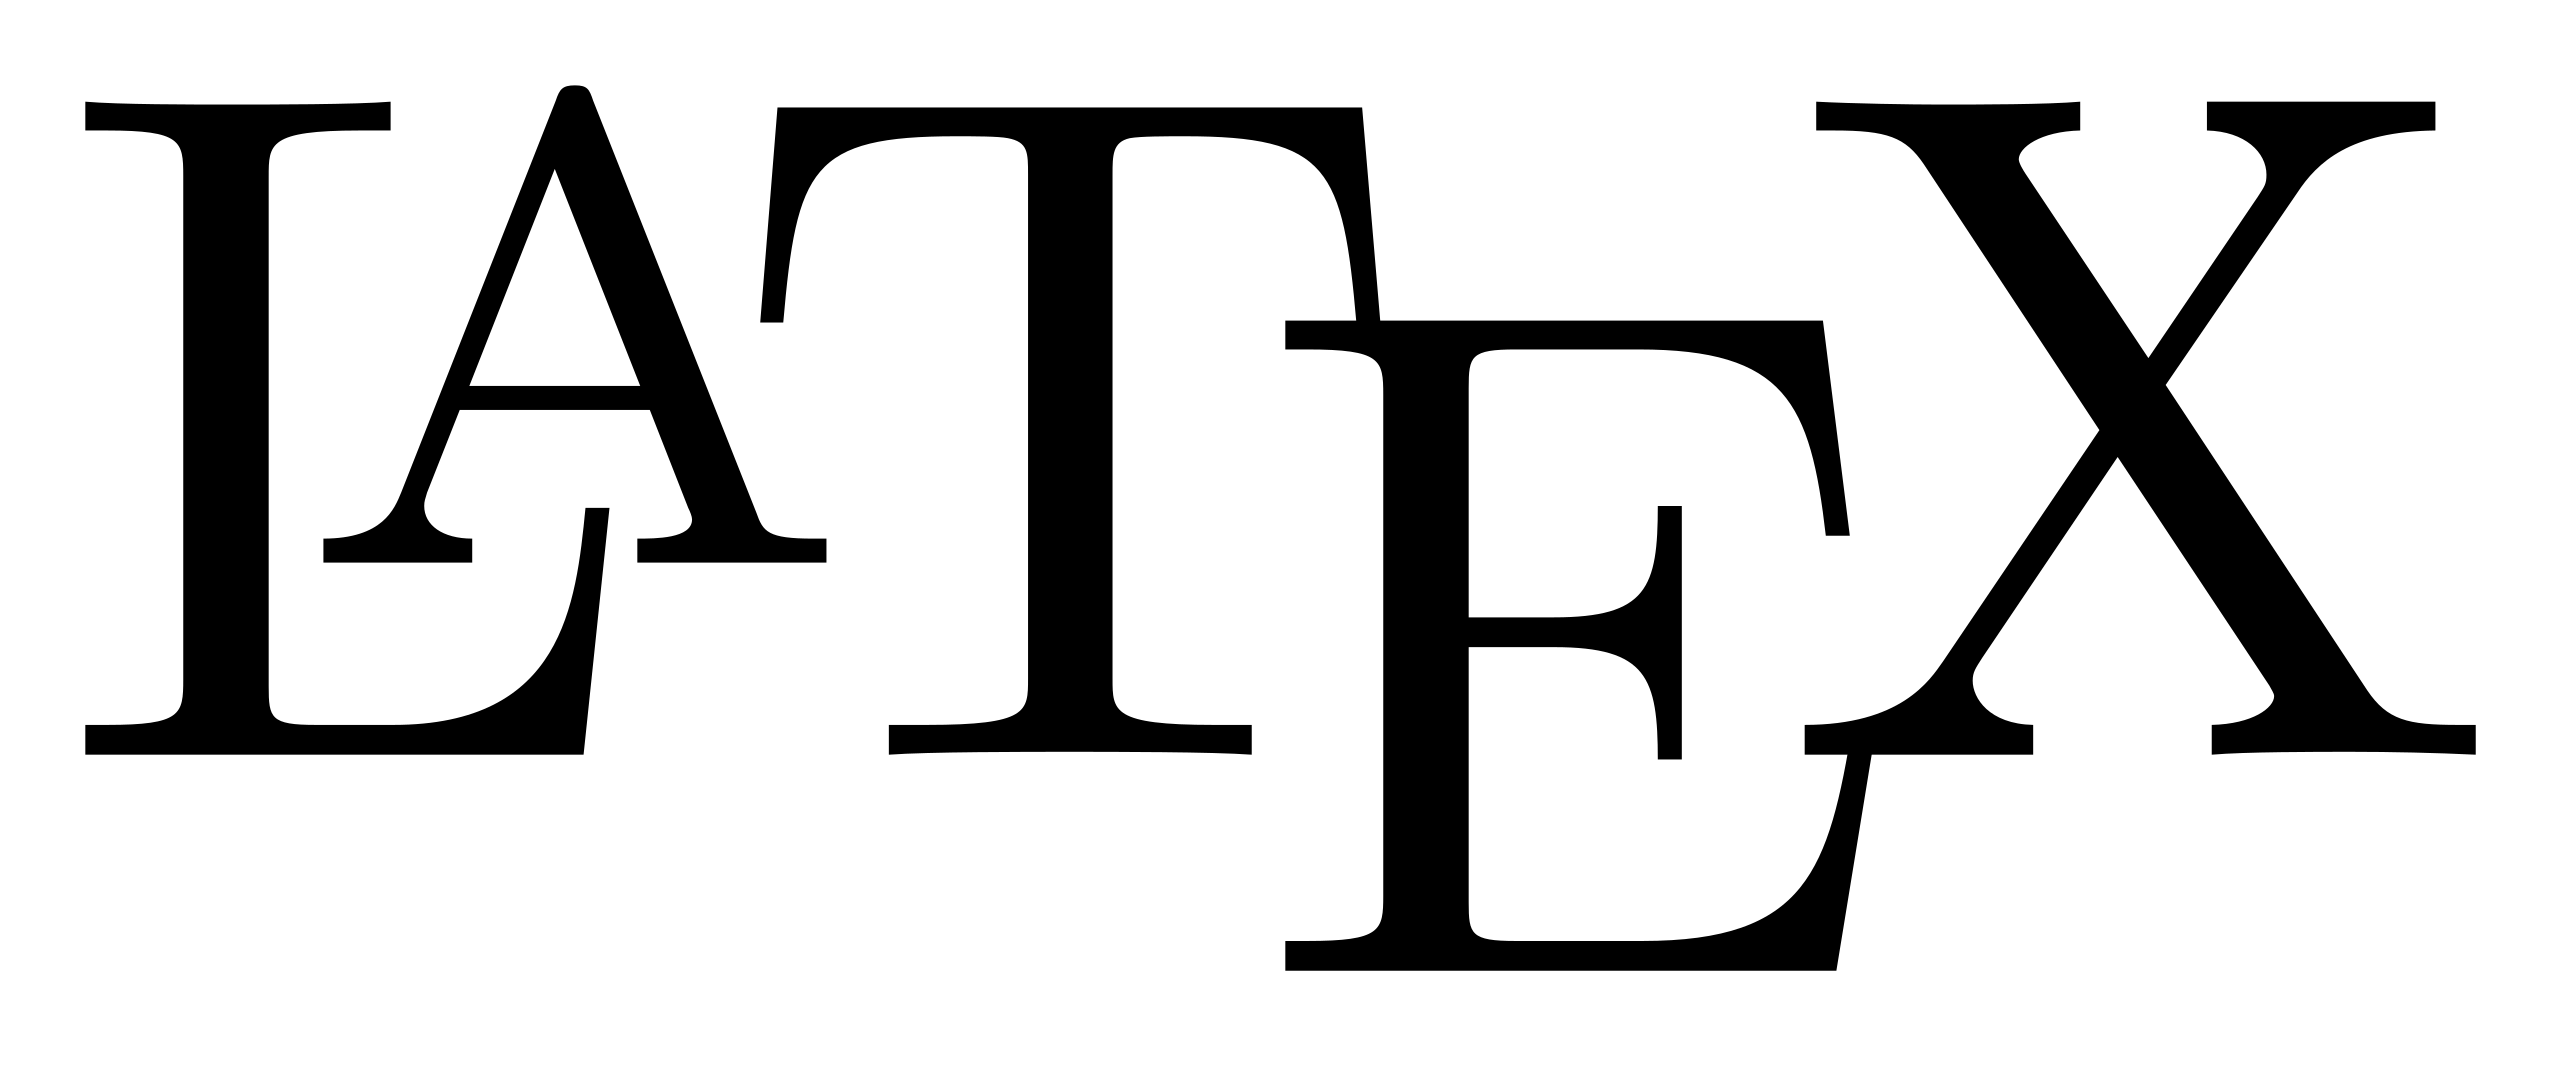
\includegraphics[height=5cm, width=5cm, keepaspectratio]{Latex}
\label{fig:eredeti}
\end{subfigure}

\begin{subfigure}[c]{5cm}
\caption{Fejre állt kép}
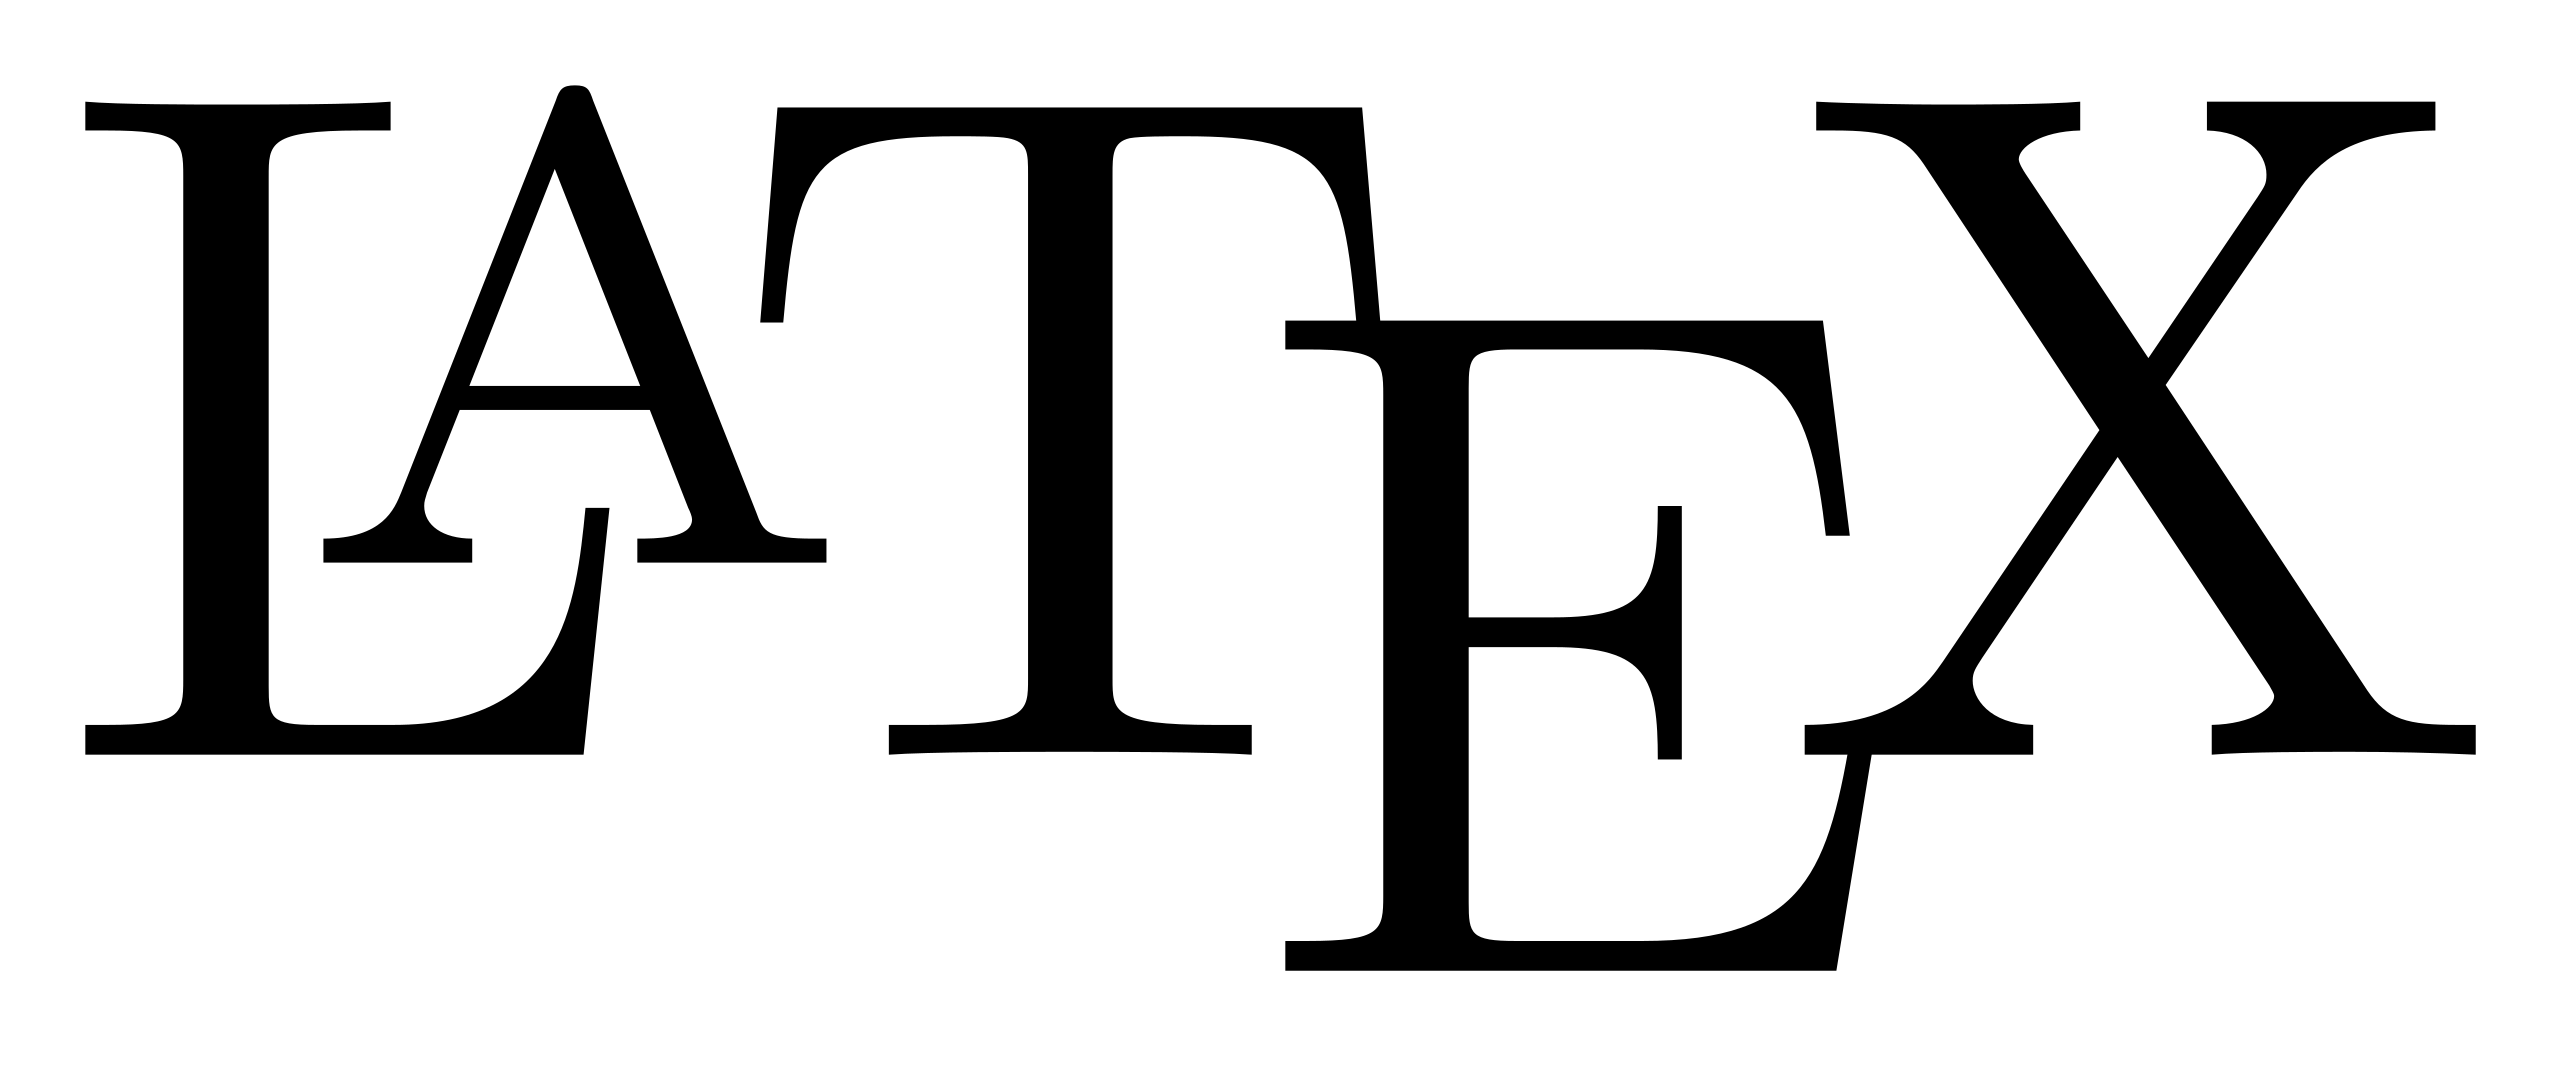
\includegraphics[angle=180, origin=c, height=5cm, width=5cm, keepaspectratio]{Latex}
\label{fig:fejenallo}
\end{subfigure}

\end{wrapfigure}
\hulipsum

\ref{fig:kepek}
\ref{fig:eredeti}
\ref{fig:fejenallo}


\subref{fig:eredeti}
\subref{fig:fejenallo}

\end{document}